\documentclass[a4paper,12pt,final]{report}  

\usepackage[utf8]{inputenc}
\usepackage[abspath]{currfile}
\usepackage[czech]{babel}
\usepackage{booktabs}
\usepackage{xcolor}
\usepackage{watermark}
\usepackage{graphicx}
\usepackage{transparent}
\usepackage{tikz}
\usepackage{fontspec}
\usepackage{styl}
\usepackage{array}
\usepackage{hyperref}
\usepackage{tabularx}
\usepackage[margin=1cm,footskip=-3cm]{geometry}
\usepackage{smartdiagram}

\hypersetup{
    colorlinks=false,
    linktoc=all,
    pdftitle={T.O.Severka - Školení táborových vedoucí 2022},
    pdfauthor={Daniel Adámek a tým T. O. Severka},
    pdfkeywords={školení, metodiky, pedagogika, motivace, koučování, příprava}
    }

%opening
\begin{document}
\author{Daniel Adámek}
\begin{titlepage}

\mainpagelogo

\centering 
        \Large{Česká Tábornická Unie z. s.}
        \vspace{0.5cm}
        
        \Large{T. O. Severka p. s.,}
        \vspace{7.5cm}
        
        \Huge
        \textbf{Školení táborových vedoucí pro rok \the\year{}}
            
        \vspace{1.5cm}
            
        \large{Vypracoval tým T. O. Severka}
            
        \vfill
        \today

        \vspace{0.8cm}
\end{titlepage}

\pagebreak

\newpage

\

\newpage

\tableofcontents
\pagelogos
\pagebreak

\chapter{Lidé}\pagelogos
\section{Lidé mají různé potřeby}
Pokud chceme s lidmi pracovat, musíme porozumět jejich potřebám a ty jsou úzce svázány s motivací. Pokud mám určitou potřebu, jsem motivován k činnosti, která vede k uspokojení této potřeby (například hlad a lov). Platí to také naopak.
Pokud do motivace vložíme dostatečné úsilí a prostředky, můžeme lidi motivovat k ledasčemu, nicméně nejsnazší je lidi motivovat k uspokojení jejich (často podvědomých) potřeb.

Jaké jsou lidské potřeby? Schematicky je vyjadřuje známá Maslowova pyramida potřeb. Jednoduše platí: aby se projevila vyšší patra pyramidy potřeb, musí být uspokojena nižší patra.

\begin{samepage}

\vspace{1cm}
\textbf{Maslowova pyramida potřeb}

Pyramida potřeb má důležité důsledky pro zážitkové akce. Pokud chceme řešit hlubší problémy, musíme účastníky nejdříve nakrmit, nechat je vyspat a dát jim možnost uspokojit základní hygienické potřeby.
\begin{figure}
\pagelogos
\begin{center}
    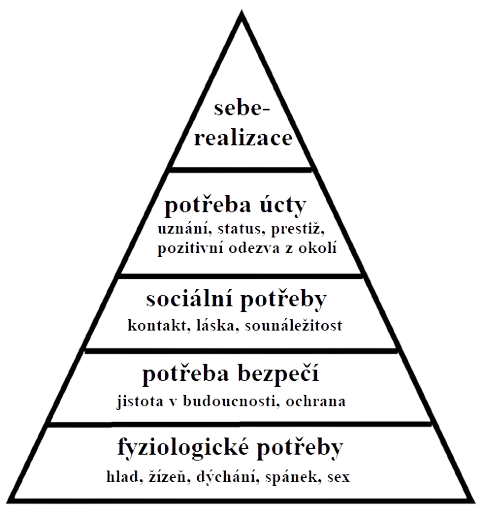
\includegraphics[width=0.9\textwidth]{zdroje/maslowova-pyramida-lidskych-potreb.png}
    \caption{Maslowova pyramida potřeb}
\end{center} 
\end{figure}
\end{samepage}

\section{Lidé jsou různí}
\pagelogos
Lidé jsou různí. Zní to sice jako triviální fakt, ale lidé podvědomně promítají do ostatních sebe. Jak praví přísloví: \textit{Podle sebe soudím tebe.} A tak se stává, že předpokládáme, že ostatní vnímají situaci stejně jako my, a že se budou chovat stejně jako my.
Jenže oni se často chovají úplně jinak a dochází ke zbytečným nedorozuměním.
K uvědomnění si rozdílnosti lidí slouží typologie osobnosti. Typologie nám pomáhají ujasnit si, jací jsme my a v čem všem se od nás ostatní mohou odlišovat. Je třeba si pamatovat, že žádná typologie není absulitní a každý člověk je specifickou kombinací různých typú. Lidé nejsou černobílí, lidé jsou složití!
\begin{samepage}
\subsection*{Typologie}
Tato typologie kombinuje čtyři charakteristiky:
\begin{itemize}
 \item Přístup k okolnímu světu\\
    \textbf{extrovert} x \textbf{introvert}\\
    \textbf{Extrovert} je otevřený, rád se pohybuje mezi lidmi, hodně mluví, přemýšlí během hovoru. \textbf{Introvert} je uzavřený, má odstup od okolí, víc naslouchá, než mluví a když mluví, tak si rozmyslí dopředu, co řekne.
    
 \item Příjem informací\\
    \textbf{smyslový} x \textbf{intuitivní}\\
    \textbf{Smyslový} typ lidí přijímá realitu, přítomnost, detaily, přesnost, osvědčené postupy. \textbf{Intuitivní} typ lidí přijímá představivost, budoucnost, vize, obecný přehled, inovace.
 \item Zpracování informací\\
    \textbf{myšlení} x \textbf{cítění}\\
    Lidé zpracovávající informace \textbf{myšlením} upřednostňují logické myšlení, racionalitu, přesné analýzy, objektivitu, spravedlnost. Lidé zpracovávající informace \textbf{cítěním} věnují pozornost citům, vztahům, porozumění, soucitu, postojům.
 \item Rozhodování se\\
    \textbf{vnímající} x \textbf{usuzující}\\
    \textbf{Vnímající} lidé jsou impulzivní, mají rádi proměnlivost, nevázanost, nepříjemné věci odkládají, příliš neplánují, dodělávají věci na poslední chvíli. \textbf{Usuzující} lidé jsou pečliví, plánují, mají rádi jasné závazky a systematické chování, nepříjemné věci raději řeší hned.
\end{itemize}
\end{samepage}\pagelogos
\begin{samepage}\begin{flushleft}
\fbox{%
    \parbox{0.977\linewidth}{
        \textbf{Úkol!} Jak byste charakterizovali sebe? Dá se to nějak poznat?
    }
}
\end{flushleft}
\textbf{Místo pro poznámky}
\vspace{3cm}\pagelogos
\end{samepage}

\subsection*{Motivační založení}
Jako další typologii uvedeme souvislost s motivací. Podobných typologií můžeme najít více, zmíněná je jedna z verzí.

\begin{itemize}
 \item \textbf{Objevovatelé}. Hledají výzvy, překonávají překážky, jsou netrpěliví, tvořiví, přichází s originálními myšlenkami. na pochvali i kritiku reagují smyslem "já vím". \\
 \textit{Motivace:} je to těžký úkol, udělej to, jak chceš. \\
 \textit{Demotivace:} rutina, jedoduché, přesně dané postupy.
 
 \item \textbf{Usměrňovatelé}. Usilují o vliv na své okolí. Jsou rádi středem pozornosti, rádi vedou druhé. Kritiku neradi slyší.\\
 \textit{Motivace:} je to důležité, závisíme na tobě, vezmi si lidi a zorganizuj to.\\
 \textit{Demotivace:} bagatelizace úkolu nebo osobní důležitosti.
 
 \item \textbf{Slaďovatelé}. Zajímají se o lidi, umí naslouchat, rádi pracují v týmu, vytváří příznivé prostředí. Pochvalu převádí na ostatní, kritiku přijímají.\\
 \textit{Motivace:} budeš členem týmu, pomůžeš ostatním.\\
 \textit{Demotivace:} bojí se odpovědnosti, samostatnosti, tvořivosti.
 
 \item \textbf{Zpřesňovatelé}. Zaměřují se vždy na jednu věc a pokoušejí se dosáhnout dokonalosti. Na pochvalu příliš nereagují, ale vnitřně je velmi potěší.\\
 \textit{Motivace:} tady máš přesné instrukce, poradím ti, kdyby byl problém.\\
 \textit{Demotivace:} chaos, nutnost sociální komunikace.
\end{itemize}

\subsection*{Zájmy}
\pagelogos
Z pohledu zážitkových akcí můžeme lidi rozdělit do čtyř základních zájmových skupin. Opět nejde o jasné rozškatulkování, každý člověk v sobě kombinuje unikáním způsobem různá zaměření.

\begin{itemize}
 \item \textbf{Sportovci}. Mají dobrou fyzičku, jsou obratní, mají rádi sporty, závody, fyzicky náročné aktivity, pohyb venku. Upřednostňují jednoduchá pravidla a rychlé tempo. Motivuje je výzva
 
 \item \textbf{Stratégové}. Umí dobře logicky myslet, mají rádi týmové hry náročné na komunikaci a koordinaci. Užijí si složité strategické hry, u nichž vysvětlování pravidel zabere aspoň půl hodiny a u kterých lze vymýšlet různé finty.
 
 \item \textbf{Psychologové}. Zajímají je hlavně lidi. Mají rádi psychologicky náročné hry, diskuze, reflexe, ale i volnější program, při nemž si mohou popovídat s ostatními.
 
 \item \textbf{Umělci}. Rádi tvoří, umí hrát na hudební nástroj nebo dobře malují. Baví je tvořivé aktivity, tajemno a hry se silnou atmosférou.
\end{itemize}

Rozdělení podle zájmu můžeme využít při skladbě programu. Pokud nemáme akci omezenou  na jednu zájmovou skupinu, kombinujeme hry tak, aby si každý přišel na své. Je vhodné si položit otázku, zda-li je dobré aby tuto hru/aktivitu vykonával konkrétní člověk.

\begin{samepage}\begin{flushleft}
\fbox{%
    \parbox{0.977\linewidth}{
        \textbf{Úkol!} Zkuste se zamyslet a diskutovat nad tím, jak budou následující hry bavit jednotlivé zájmové skupiny: \textit{Vybíjená, městečko Palermo, Riskuj!, lanová dráha, výroba erbu/vlajky}
    }
}
\end{flushleft}
\textbf{Místo pro poznámky}
\vspace{3cm}\pagelogos
\end{samepage}

MBTI typologie kombinuje ještě více vlastností člověka. Pro přesnost a správný chod týmu, jak v práci, tak jinde, je třeba si znát svou typologii navzájem. K tomuto perfektně slouží stránka \textit{16personalities.com}. Testování těchto vlastností je jednou z nejčastějších rad pro velké týmy, jak zorganizovat a určit role v týmu.

\section[Lidé se s časem mění]{Lidé se s časem mění}
\pagelogos
\textit{Všichni dospělí byli nejdřív dětmi. Ale málokdo si to pamatuje. (A. S. Exupéry)}

\begin{samepage}
Vývoj člověka se dělí do několika fází:
\begin{itemize}
 \item Věk batolecí: Jsem to, co mohu svobodně dělat.
 \item Věk předškolní: Jsem to, co učiním.
 \textbf{
    \item Věk školní: Jsem to, co dovedu.
    \item Věk dospívání: Jsem to, co čemu věřím.
    \item Věk mladé dospělosti: Jsem to, co miluji.
 }
 \item Věk střední: Jsem to, co poskytuji.
 \item Věk zralosti: Jsem to, co po mně zůstane a přežije.
\end{itemize}
\end{samepage}

U nás bude potřeba znát jen ty tři prostřední kategorie. Základní charakteristiky jsou uvedeny v tabulce, která dává přehled toho, co baví a nebaví děti, dospívající a mladé dospělé. Kromě charakteristik uvedených v tabulce stojí za zmínku vztah k samostatnosti a autoritě. \textbf{Děti} jsou velmi nesamostatné, nerady vyvíjejí vlastní iniciativu, musíme jim přesně zadat, co mají dělat. Vůči autoritám mají děti respekt a poslouchají je. \textbf{Dospívající} jsou schopni samostatné činnosti a vlastní iniciativy, ale příliš se k tomu nemají a musíme je popohánět. Ve vztahu k autoritám jsou vyzývaví a neradi se podřizují. \textbf{Dospělí} jsou samostatní a mají rádi volnost. Vlastní iniciativy jsou schopni jenom občas potřebují "nakopnout". Autority poslouchají, ale nemají rádi, pokud si s nimi někdo nedá práci nebo pokud mají pocit, že jsou autoritou zneužíváni.

\begin{center}
\renewcommand{\arraystretch}{1.5}
\begin{tabular}{ | m{2cm} || m{4.2cm}| m{4.2cm} | m{4.2cm} | } 
  \hline
  & \vspace{.3cm} \textbf{VĚK ŠKOLNÍ} & \vspace{.3cm} \textbf{VĚK DOSPÍVÁNÍ} & \vspace{.3cm} \textbf{VĚK MLADÉ DOSPĚLOSTI}\tabularnewline [12pt]
  \hline
  \textbf{HLEDAJÍ} & kamarády, zábavu & skupinu, srovnání & partnera, odpovědi, sebepoznání\tabularnewline
  \hline
  \textbf{MAJÍ RÁDI} & akce, boj, noc, dobrodružství, bodování & akce, sport, recese, emoce & rozmanitost, náročné úkoly, smysluplnost \tabularnewline
  \hline
  \textbf{NEMAJÍ RÁDI} & náročné úkoly, přemýšlení & příliš filozofování, příliš náročné úkoly & samoúčelnou činnost, bodování \tabularnewline
  \hline
  \textbf{NÁMĚTY} & pohádky, dobrodružné příběhy, fantazie, indiáni & fantasy světy, historie (akční prvky), tajemno & lidi, vztahy, historie (filozofické prvky), současnost \tabularnewline
  \hline
  \textbf{SOUTĚŽENÍ} & soutěží rádi, spolupráce jim nejde & raději soutěží, nutnost spolupráce si uvědomují & občas si zasoutěží, ale rádi spolupracují \tabularnewline
  \hline
  \textbf{ÚNAVA} & malá výdrž, rychlá regenerace & střední výdrž i regenerace & velká výdrž, pomalá regenerace \tabularnewline
  \hline
  \textbf{METAFORY} & nechápou & nechce se jim nad nimi přemýšlet & chápou a mají rádi \tabularnewline
  \hline
\end{tabular}
\end{center}
\pagelogos

Čím mladší a méně zkušení jsou účastníci, tím \textbf{konkrétnější a jasnější informace} jim musíme dávat. Tento princip je třeba aplikovat na všechny oblasti: příběh, pravidla her, kladení otázek, zadání tvořivých aktivit.


\section[Lidé ve skupině]{Lidé ve skupině}
\pagelogos
\textit{Člověk je jediný tvor, který se červená. Nebo by alespoň měl. (M. Twain)}

V předchodí části jsme se zabývali lidmi jako jednotlivci. Ovšem člověk je tvor společenský a značnou část svého života tráví interakcí s ostatními. Pro zážitkové akce to platí obvzlášť, protože na nich dochází k interakci mezi lidmi téměř neustále.

\subsection*{Komunikace}
Dobrá komunikace je pro zážitkové akce klíčová, predevším co se týče komunikace uvnitř vedoucovského týmu. Většina sporů mezi instruktory, nemá původ v rozdílných názorech nebo selháních, ale v komunikaci.

\textbf{Základní pravidlo:} Není důležité, co říkáme, důležité je, co ostatní slyší. Bohužel to není jednoduché dosáhnout toho, aby ostatní slyšeli právě to, co chceme řáct. Několik rad vhodných pro zvlášť vypjaté situace:

\begin{itemize}
 \item Komunikace má být vedena s dobrými úmysly. Měli bychom si být jistí vlastní motivací. Není účelem jen namíchnout druhého?\\
 \textit{"Celou hru jste úplně zkazili, jasně jsem říkal, že jim do toho sklepa máte napustit 10cm vody, a vy jste tam napustili aspoň 15cm, tak není divu, že jim natelko do bot a teď jsou naštvaní."}
 
 \item Komunikace má být upřímná, konkrétní a aktuální. Říkám, co si opravu myslím, co je relevantní pro daný okamžik, a říkám to co nejjasněji. Nevytahuji staré křivdy. Mluvím za sebe, nezobecňuji.\\
 \textit{"Všichni si beztak myslí, že chceš pořád jenom hrát hry ve sklepě a vůbec nevím, k čemu to je."}
 
 \item Pro komunikaci vybíráme vhodný okamžik. Sporné záležitosti řešíme v soukromí (rozhodně ne před účastníky - dětmi) a ve chvíli, kdy nejsme zaneprázdněni jinou činností.\\
 \textit{"Pepo, mohl bys na chvíli přestat balit Evu?; Musím ti říct, proč si myslím, že ta tvoje hra byla úplný propadák."}
\end{itemize}

Důležitou součástí dobré komunikace je naslouchání. Když mluví druhý, dobře poslouchám, co mi říká, a nepřemýšlím, co řeknu já. Snažím se přemýšlet nad jeho slovy. Když mi to říká, asi to tak vnímá. Není dobré se hned začít bránit a všechno vysvětlovat. Měl bych pořádně poslouchat, rozhodně všek naní dobré hned všechno zohledňovat. Každopádně bych měl na sdělení druhého vždy reagovat, dát najevo, že jsem poslouchal a že se nad sdělením zamyslím.

Důležitou součástí projevu je také neverbální komunikace, do které patří například postavení těla, mimika, gesta nebo postavení v prostorů. Podle neverbálních prvků komunikace se často pozná neupřímnost či lež.

\section[Úhel pohledu]{Úhel pohledu}
\pagelogos
Každý člověk má v hlavě mnoho různých tzv. mentálních map. Každou z těchto map můžeme přiřadit do jedné ze dvou základních kategorií: mapy popisující \textit{věci takové, jaké jsou (realita)}, nebo mapy, popisující \textit{věci takové, jaké by měly být (hodnoty)}. Všechno s čím se v životě setkáváme, interpretujeme pomocí těchto mentálních map. Jenom málokdy se přitom zabýváme tím, zda jsou přesné. Obvykle si totiž ani neuvědomujeme jejich existenci. Jednoduše předpokládáme, že věci jsou nebo by měly být takové, jaké je vidíme, jak je známe.
Z těchto přepokladů vyrůstají naše postoje a chování. To jak myslíme a jednáme, má svůj zdroj tom, jak vidíme věci kolem sebe.

\newpage
\begin{flushleft}
\fbox{%
    \parbox{0.977\linewidth}{
        \textbf{Úkol!} Podívejte se na první obrázek (nejlépe si přeložte stránku tak, ať nevidíte další obrázky).\\
        Poté se podívejte na druhý obrázek a pečlivě popište, co na něm vidíte.\\
        \textbf{Je to žena? Jak je asi stará? Jak vypadá? Co má na sobě? Jaké postavení a životní role byste jí přisoudili?}
    }
}
\end{flushleft}

\begin{figure}[h]
\begin{center}
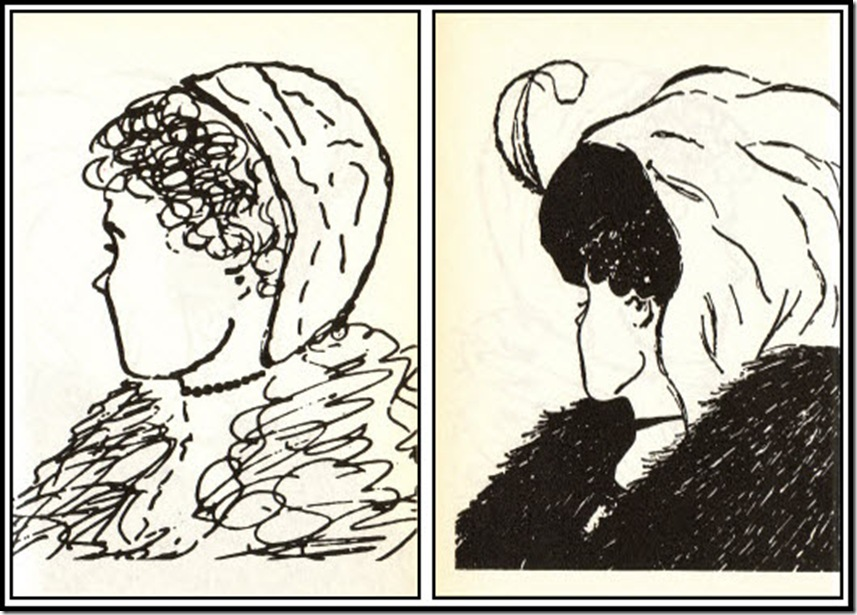
\includegraphics[width=0.75\textwidth]{zdroje/POV-young.jpg}
\caption{První obrázek úhlu pohledu}
\end{center}
\end{figure}


\vspace{5cm}

\newpage
\begin{figure}
\begin{center}
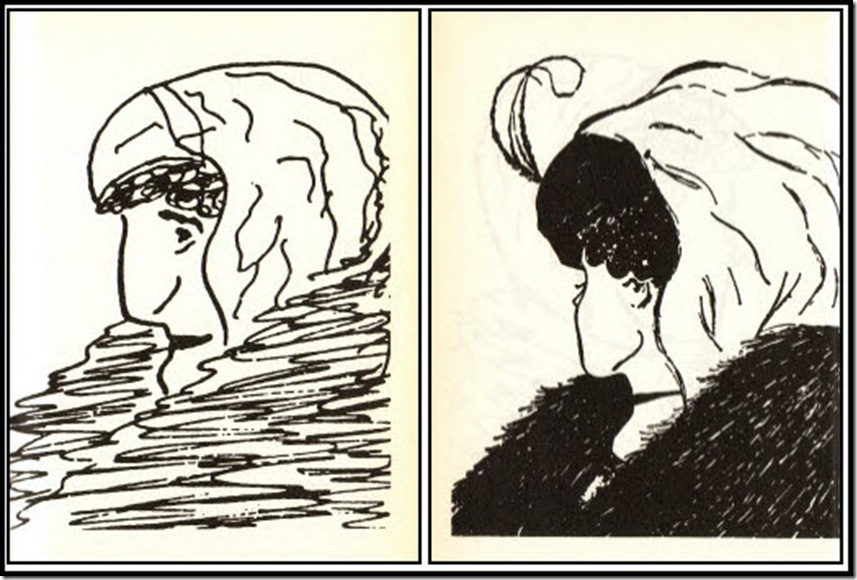
\includegraphics[width=0.75\textwidth]{zdroje/POV-old.jpg}
\caption{Druhý obrázek úhlu pohledu}
\end{center}
\end{figure}

\pagelogos
\section[Experimenty]{Experimenty}
\subsection[Experiment Třetí vlna]{Experiment Třetí vlna}
\label{Experiment-Treti-Vlna}
Experiment proběhl během jednoto týdne roku 1967 na Cuberley High School v kalifornském města Palo Alto. Nevedl ho psycholog, či psychiatr - ale učitel historie Ron Jones. Ten chtěl studentům druhého ročníku přihlážit situaci při nástupu nacismu v Německu.

\textbf{První den} experimentu museli studenti pouze vzorně sedět, komunikovat vstoje, své odpovědi vměstnat maximálně do tří slov a začínat je oslovením "pane Jonesi". Učitel jim také zdůrazňoval sílu disciplíny a jednoty

\textbf{Druhý den} Jones pojmenoval osazenstvo třídy hnutím Třetí vlna a stanovil speciální pozdrav, jímž se "členové hnutí" museli zdarvit i mimo třídu.

\textbf{Třetí den} začal žít experiment svým vlastním živote. K hnutí přibyli další studenti, Jones jim rozdal karty se speciálními úkoly, též je instruoval, jak "lovit" nové členy, třem studentům pak dal speciální průkazky - měli donášet na ty, kteří pravidla nedodržují. Jenže dobrovolně donášelo dalších 20 studentů. Na konci třetího dne mělo hnutí na 60 účastníků a někteří studenti dokonce těm spolužákům, kteří nedodržovali pravidla, vyhrožovali.

\textbf{Čtvrtý den} se experiment vymkl kontrole, studenti se do experimentu zcela ponořili a jejich loajalita byla perfektní, přibyli i další členové. Jones oznámil, že jejich buňka je součástí celonárodního hnutí, které má změnit americkou společnost a v pátek v poledne bude jeho existence a síla demonstrována v televizi.

\textbf{Pátý den} přišlo do stanovené místnosti přes 200 lidí, nechyběli transparenty, studenti skandovali oficiální heslo. Žádné televizní prohlášení se však nekonalo. Naopak jim Jones oznámil, že \textit{absolvovali experiment, při němž se chovali stejně, jako přívrženci nacismu} v Německu a že všechno co jim řekl byla lež.

\textbf{\Large \flushleft Co nám z toho vyplývá?} Skupina ovlivňuje chovájí svých členů.

\subsection[Stanfordský vězeňský experiment]{Stanfordský vězeňský experiment}
K šokujícím výsledkům došel v roce 1971 i Philip G. Zimbardo ze Stanfordovy univerzity. Ten tehdy vybral 24 zcela zdravých studentů ze 75 přihlášených dobrovolníků, kteří měli žít ve vězení. Někteří z nich měli být vězni bez jakýchkoliv práv, jiní dozorci. Zimbardo musel experiment předčasně ukončit; vymkl se mu totiž z rukou, když \textit{"dozorci" začali "vězně" ponižovat způsobem, který jim mohl způsobit trvalé následky}.

\textbf{\Large \flushleft Co nám z toho vyplývá?} Zdravý a rozumně smýšlející člověk, je-li vystaven extrémním podmínkám, se může radikálně změnit (nebo změnit své chování). A to velmi v krátké době, viz \nameref{Experiment-Treti-Vlna}.

\newpage
\pagelogos
\chapter{Práce vedoucího}
Aby nedocházelo k nedopatřením, musíme včas vymyslet funkční systém. Proto je třeba vytvořit základní pravidla a operační principy.

\textbf{Základní pravidla jsou pravidla vytvořená vedoucími pro účastníky.} 
Vedoucí očekává, že budou daná pravidla respektovat, neboť jinak by nebylo možné tato pravidla využívat. Vyhlašují se na začátku akce. Jsou viditelně umístěna a dostupná každému.

\textbf{Operační principy jsou pravidla vytvořená účastníky pro ně samé}
Reprezentují způsob, jakým účastníci očekávají, že se sami k sobě během programu budou chovat. Jsou také vytvořena na začátku projektu, ale vlastními účastníky projektu. Jsou opět viditělně umístěna a dostupná každému.

\textbf{Oba tyto druhy pravidel je třeba s účastníky stanovti hned na úvod akce. Je to důležitý a vlastně klíčový okamžik celé akce.}
Definovanými pravidly se vytváří systém žití a vztahování se na vlastní akci po dobu její trvání.

\section{Pravidla zkušeného vedoucího}
\begin{enumerate}
 \item \textbf{Když jeden mluví, ostatní naslouchají} \\
 komunikace je jednokánálová. Když mluví jeden, ostatní naslouchají. Jinak se nedomluvíme. Máme dvě uši a jedna ústa.
 \item \textbf{Respekt}\\
 chovám se k druhému tak, jak chci aby se i on choval ve stejné situaci ke mně.
 \item \textbf{Mohu mít názor, můžu se ptát} \\
 máte právo říct, co si myslíte a máte právo za to nebýt vysmívání. Něco takového jako absolutní pravda neexistuje. Obvykle máme každý svojí verzi příběhu. Je dobré mít možnost, říct svou verzi a to i ostatní.
 \item \textbf{Oslovení}\\
 je třeba se domluvit, jak se budeme oslovovat. My si všichni tykáme. 
 \item \textbf{Pochopení stačí}\\
 nemusíte s každým souhlasit. Snažte se "jen" pochopit druhé lidi. To stačí.
 \item \textbf{Zpětná vazba} \\
 můžete požádat o zpětnou vazbu a také ji můžete poskytnout. Je to jen chtěné.
 \item \textbf{Pravidlo čtyř stěn} \\
 to, co se řekne v budově a uvnitř týmu, zůstává mezi námi. Pravidlo, které se vždy porušuje a nedodržuje. Takže platí: když mluvím, tak jako by ten, o kom mluvím, stál vedle mě.
 \item \textbf{Vypněte mobily} Netřeba více komentovat.
\end{enumerate}
\section{Návyky špatného vedoucího}\pagelogos
\begin{enumerate}
 \item \textbf{Názorová nekonzistence} \\
 říká něco jiného, než si myslí; dělá něco jiného, než říká; protiřečí si.
 \item \textbf{Nepřebírá odpovědnost} \\
 nechopí se příležitosti; ponechává iniciativu na ostatních; schovává se za druhé.
 \item \textbf{Neústupnost, přesvědčení o vlastní pravdě} nepřiznává chybu.
 \item \textbf{Svéhlavá sólovost} \\
 okázalá samostatnost; odmítání/nepřijímání pomoci.
 \item \textbf{Manipulace, demagogie} \\
 předkládá manipulativní argumenty; vede zákulistní jednání; trvá na svých demagogických postojích.
 \item \textbf{Necitlivost, sociální tupost} \\
 necitlivě reaguje na projevy a chování druhých; zesměšňuje ostatní; narušuje projev, vystupování druhých.
 \item \textbf{Sólový projev, rivalita} \\
 (skrytě) soupěří o moc; pracuje jen na sebe; nepomáhá druhým.
 \item \textbf{Sebestřednost, zahleděnost do sebe} \\
 okázalost vlastního projevu; naučená, teatrální gesta; účelový nesouhlas, nepř. pro vlastní zviditelnění; nepřijímání zpětné vazby.
 \item \textbf{Přehnané sebevědomí, nesebekritičnost} \\
 přesvědčení o správnosti vlastních názorů; neochota k diskuzi.
 \item \textbf{Neprojebuje názory} \\
 opakovaná a setrvalá mlčenlivost; projevuje se jako poslední; projevuje se až na vyzvání; nepředkládá/neodkrývá své názory druhým.
\end{enumerate}\pagelogos




\newpage
\pagelogos
\chapter{Pedagogika}
\subsection*{Obecně}
Mezi nejdůležitější pojmy v pedagogice patří:
\begin{itemize} 
 \item \textbf{výchova} - hlavní prostředek socializace; je proces záměrného působení na osobnost člověka s cílem dosáhnout pozitivních změn v jeho vývoji;
 \item \textbf{socializace} - proces zespolečenšťování;
 \item \textbf{vzdělávání} - proces, který probíhá po celý život, je součástí výchovy;
\end{itemize}

Během výchovy, socializace a vzdělávání se u každé osobnosti rozvíjejí:
\begin{itemize} 
 \item \textbf{znalosti} - osvojené informace a učením získaná schopnost je přiměřeně užívat;
 \item \textbf{dovednosti} - učením získané schopnosti správně a úspěšně vykonávat určitou činnost:
 \begin{itemize}
  \item osvojené postupy a úkony,
  \item zmechanizovaná dovednost;
 \end{itemize}
 \item \textbf{postoje} - hodnotící vztahy k problémům (často např. morálním), nezřídka vedou k činům.
\end{itemize}

Určitě bychom neměli zapoměnout \textbf{didaktiku}. Didaktika se zabývá formami, postupy, a cíli vyučování. Co vůbec znamená "vyučovat"? Správný vyučující by měl učit hbitě, s chutí a důkladně (slova Komenského). 

\subsection*{Původ slova}
Pedagogika je slovo složené z dvou celků a to: \textbf{pais} - dítě, \textbf{agein} - vést; z toho vyplývá řecké slovo pedagogos - člověk vedoucí dítě (vzhůru, k poznání).

\textbf{Edukace} z řeckého \textbf{edukacio} - vést, vést z kvalitativně nižšího stavu do vyššího, táhnout vzhůru.

Vzdělávání v dobách antického řecka, probíhalo v rodinách, kde také končilo. Poté se děti svěřovaly vzdělanému otroku, který na základě povídání si-diskuze vedl rozhovor a vedl dítě k poznání. S postupem času vznikli "mudrcové" (vzdělanější otroci), ke kterým vzdělaný otrok (domácí) dováděl (vedl) dítě za výukou/vzděláním.

\section[Zážitková pedagogika]{Zážitková pedagogika}
\textit{Mysl není nádoba k naplnění, ale oheň k zapálení. (Plutarchos)}

Pomocí zážitkové akce výchovně působímena účastníky. Toto výchovné působení spadá do oboru zvaného zážitková pedagogika. Co to je? Jaké jsou její metody?

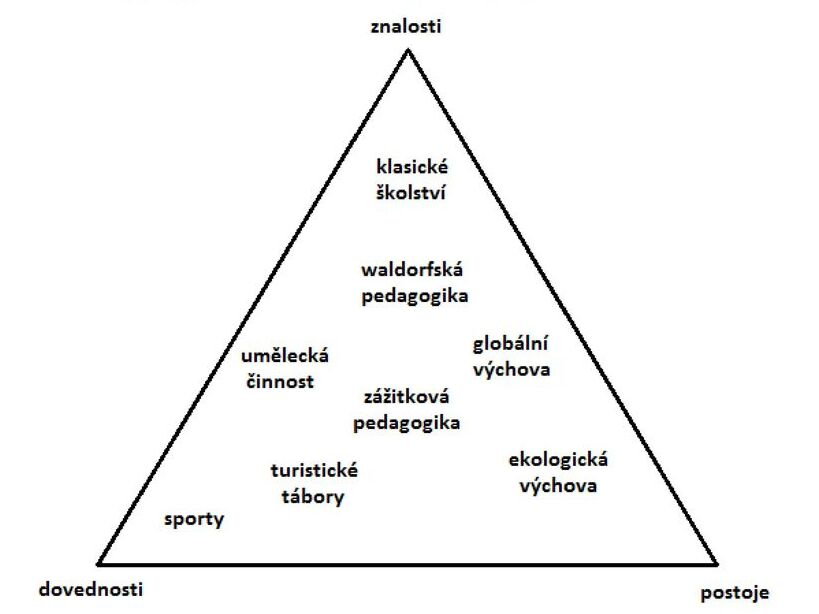
\includegraphics[width=0.75\textwidth]{zdroje/pedag-zamereni.jpg}

Prostřednictvím výchovy a vzdělávání můžeme oblivňovat tři zdroje, ze kterých pramení chování a život lidí: znalosti, dovednosti a postoje. Pedagogické směry se liší v tom, na který v těchto zdrojů se zaměřují. Obrázek je velice zjednodušující, pedagogické směry nelze takto jednoduše definovat, přechod mezi nimi je plynulý.

\subsection*{Učení se prostřednictvím zážitku}\pagelogos
\textit{Řeknimi, já zapomenu. Ukaž mi a já si možná vzpomenu. Zapoj mě a já pochopím. (čínské přísloví)}

Základem zážitkové pedagogiky je vlastní aktivita, protřednictvím které vychovávaný člověk získá zážitky. Čím víc vlastní energie musí člověk vynaložit, tím je zážitek intenzivnější, zapamatovatelnější a využitelnější pro výuku. Komerční zábava se rozptýlí, ale nezanechá žádné stopy, protože nás nestojí žádnout energii. Pokud od nás aktivita vyžaduje vysoký vklad fyzické nebo psychické energie, je sice méně lákavá, ale o to větší má potenciál.

Ovšem samotný zážitek ještě nestačí k tomu, aby se člověk něco naučil. Rozdíl mezi ``rekreačním'' zážitkem a ``pedagogickým'' zážitkem tkví v reflexi. K učení dochází díky zkoumání a zpracovávání zkušeností, které zážitek vyvolal.

Prostřednictvím zážitku samozřejmě nemůžeme zpracovávat všechna témata. Diferenciální rovnice takto asi nikoho nenaučíme. Obecně jsou pro učení prostřednictvím zážitku vhodné dovednosti a postoje, konkrétně pak sociální učení (sebepoznání, spolupráce), měkké schopnosti (práce v týmu, vedení lidí, vztahové a komunikační dovednosti), životní postoje (tolerance, odpověďnost) a metody řešení problémů (kritické myšlení).


\section[Výchova]{Výchova}\pagelogos
Výchova není jen jednoduchá operace: přikazování, zakazování, doporučování, vysvětlování, přesvědčování (jak se může zdát). Jedná se o komplexní činnost, která dlouhodobě formuje člověka a záměrně usiluje o "vytvoření" člověka vyznačujícího se co nejlepšími vlastnostmi, schopnostmi a předpoklady k plnohodnotnému dospělému životu.

\begin{samepage}\begin{flushleft}
\fbox{%
    \parbox{0.98\linewidth}{
        \textbf{Úkol!} zamyslete se nad otázkami: \textit{"K čemu je výchova dobrá?"} Jakou \textbf{funkci} má?
        \small{
        \begin{enumerate}
        \item pro každého z nás?
        \item pro společnost jako celek?
        \end{enumerate}}
    }%
}
\end{flushleft}
\textbf{Místo pro poznámky}
\vspace{5cm}\pagelogos
\end{samepage}

\textbf{Výchova} je proces, který umožňuje jedincům se plnohodnotně zapojit do života ve společnosti. Připravuje člověka pro plnění několika společenských rolí, které na něho v životě čekají. Zároveň umožňuje předání kultury (tradice) z jedné generace na další, čímž zabezpečuje kontinuitu společenského vývoje.

\textbf{Rysy výchovy:}
\begin{itemize}
 \item vnější ovlivňování pozitivního rozvoje člověka,
 \item záměrné, cílevědomé působení na člověka,
 \item interakce vychovatele a vychovávaného,
 \item předávání kultury lidstva dalším generacím,
 \item zhodnocování vnitřních předpokladů člověka.
\end{itemize}

Výchova jakožto proces (dlouhodobý i krátkodobý) má vždy nezbytné etapy:
\begin{itemize}
 \item počáteční etapa - \textbf{diagnóza} - je nezbytné poznat stav, úroveň vychovávaného (vychovávaných);
 \item etapa pedagogického \textbf{projektování} - vymezení a formulace konkrétních nebo obecnějších cílů, postupů;
 \item etapa \textbf{regulace učení} vychovávaných - výchova je vždy subjektivně učení, jde tedy o motivaci, konkrétní obsah činnosti, fixování osvojených obsahů;
 \item etapa \textbf{výsledné} pedagogické \textbf{diagnózy} - zjišťování výsledků porovnáváním s vymezeným cílem + analýza procesu výchovy z hlediska dosažených výsledků.
\end{itemize}

\begin{figure}[ht!]
\centering
\smartdiagram[circular diagram:clockwise]{
    Obecný cíl výchovy,
    Dílčí cíle výchovy,
    Podmínky realizace cílů výchovy,
    Základní prostředky výchovy,
    Výsledky výchovy}
\caption{Cyklický proces výchovy}
\end{figure}\pagelogos

\subsection*{Cíle výchovy}
\pagelogos
Vycházíme-li z pojetí výchovy jako \textbf{záměrného, cílevědomého působení} na rozvoj osobnosti, považujeme cíl výchovy za kategorii, která významně určuje celý proces i konkrétní průběh výchovy. Již Komenský formuloval \textit{"Cíle si všímej bedlivěji než prostředků!"}

Výchovný cíl je tedy to, čeho chceme dosáhnout výchovnými úkony. Každopádně je to určitá vlastnost, nebo souhrn více vlastností osobnosti, která je objektem výchovy. Může jít o relativně speciální vlastnost (např. schopnost číst s porozuměním) nebo určitý stav celé osobnosti (např. schopnost spolupracovat s lidmi).

Abychom si mohli formulovat a vymezovat cíle výchovy, je třeba si uvědomit (vědět a znát), které kvality člověka, osobnosti jsou \textbf{naučitelné}, které tedy můžeme výchovou ovlivnit, kterých lze vhodnou výchovou dosáhnout.

\textbf{Druhy cílů}
\begin{itemize}
 \item \textbf{kognitivní} - rozvoj poznání a poznávacích schopností,
 \item \textbf{afektivní} - rozvoj postojů, prožitků, emojí, hodnot.
 
 Přijímání - reagování - oceňování hodnost - integrace hodnot - začlěňování hodnot do charakteru osobnosti - postoje - sociální prožitky.
 \item \textbf{konativní} - operace, dovednosti, pohybová zdatnost
 
 Vnímání - zaměřování - řízená motorická reakce - automatizace motorických dovedností - schopnost motorické adaptace - motorická tvořivost
\end{itemize}

\subsection*{Podmínky výchovy}
Podmínky výchovy představují poměrně široký a nepřehledný soubor prvků. Výchova se vždy děje za zcela určitých situacích. V situacích \textbf{přírodních:} jaro, prší, jsme zdraví, ...; \textbf{materiální povahy:} sedíme na zahradě, kterou jsme právě uklidili, pijeme z jistých sklenic; \textbf{sociální povahy:} sedí s námi rodiče, babička, tetička, kritizující sousedovic děti.

Podmínky výchovy tedy můžeme charakterizovat jako \textbf{situace}, v rámci kterých se realizuje výchova, ale i jako situace, které usnadňují (či naopak komplikují) výchovnou aktivitu.

Podmínky mohou být dále \textbf{stabilní}, které trvají dlouhodobě a \textbf{dynamické}, které se rychle mění.

Správná výchova je organizovaná a musí počítat se všemi podmínkami a počítat s konkrétními u každého dítěte.

\begin{figure}[ht!]
\centering
\smartdiagram[bubble diagram]{ PODMÍNKY VÝCHOVY, Biologické, Psychické, Sociální}  
\caption{Podmínky výchovy}
\end{figure}\pagelogos

\begin{samepage}
\textbf{Podmínky výchovy}
\pagelogos
\begin{itemize}
 \item Biologické - \\
    \textbf{vnitřní} - stav organismu, nervové soustavy, zdravotní stav, výška, váha; \\
    \textbf{vnější} - přírodní prostředí
    
 \item Psychické - \\
    \textbf{vnitřní} - vlohy, schopnosti, emocionalita, motivace, zájmy; \\
    \textbf{vnější} - sociální skupina, životní styl a tradice
    
 \item Sociální - \\
    \textbf{makroprostředí} - politické, ekonomické;\\
    \textbf{mikroprostředí} - rodina, spolužáci
\end{itemize}
\end{samepage}

\begin{samepage}\begin{flushleft}
\fbox{%
    \parbox{0.977\linewidth}{
        \textbf{Úkol!} Napište několik sociálních podmínek, které mají většinout pozitivní a které především negativní vliv na utváření člověka. \\
        Jak vysvětlíte, že některé děti z kuřáckých rodin velmi brzy podléhají kouření a s z některých se stávají zapřísáhlí nekuřáci?
    }
}
\end{flushleft}
\textbf{Místo pro poznámky}
\vspace{5cm}\pagelogos
\end{samepage}

\subsection*{Prostředky výchovy}
Prostředkem výchovy je každý jev, proces, situace, který je \textbf{záměrně použit pro dosažení některého cíle výchovy} - obecného, konkrétního, krátkodobého, kongitivního, afektivního,... . 

Jestliže výchovu považujeme za společnou aktivitu vychovatele a vychovávaného, pak musíme prostředky výchovy chápat jako prostředky \textbf{vnější} (používané vychovatelem) a prostředky \textbf{vnitřní}, s nimiž vstupuje do procesů dosahování cílů výchovy sám vychovávaný.

Má-li výchova skutečně vést k optimálnímu rozvoji osobnosti, pak jakýkoliv vnější prostředek musí vždy počítat s určitými prostředky a s určitou mírou mobilizace, aktivizace daných vnitřních prostředků.

\subsection*{Výsledky výchovy}
Výsledky výchovy je dosažený, předem formulovaný cíl. Je třeba pracovat s výše zmíněnou cykličností výchovy.

\textbf{Hlavní body}
\begin{itemize}
 \item Zjišťujeme, zda a v jaké úrovni jsme dosáhli stanoveného cíle. Co se nepodařilo?
 \item Hodnotíme předcházející výchovu $\Rightarrow$ můžeme provést korektury, abychom v dalších krocích chyby neopakovali.
 \item Dosažené výsledky aktivně vstupují (nebo jsou záměrně vtahovány) do dalších etap výchovy (sebeučení).
 \item Vychovávaný získává zpětnou vazbu (sebepoznání, sebepochopení, sebevědomí) - má význam při procesu sebevýchovy.
\end{itemize}

\begin{samepage}\begin{flushleft}
\fbox{%
    \parbox{0.977\linewidth}{
        \textbf{Úkol!} Proč by měl vychovatel zjišťovat výsledky výchovy? Poraďte se ve skupině a zkuste vymyslet alespoň 3 důvody.
    }
}
\end{flushleft}
\textbf{Místo pro poznámky}
\begin{enumerate}
    \item 
    \item 
    \item 
\end{enumerate}
\vspace{2cm}\pagelogos
\end{samepage}

Dále je třeba si položit otázku \textbf{efektivity}. Vyplatí se to, jak jsme vychovávali? Nešlo by to lépe? Nalezená kritéria bychom také měli zahrnout do korektury našich postupů.

\section{Rozvoj člověka}\pagelogos
Správný pedagog si pro rozvíjení člověka musí promyslet své kroky.
\textit{Rodič-pedagog si je nemusí promýšlet, protože disponuje dostatečnou intuicí. Při závažnějších krocích života si i rodič musí promýšlet své kroky, jak směřovat dítě.}

\begin{itemize}
 \item \textbf{Proč?}
 
Proč vzdělávat, co je cílem mého vzdělávání, jak cíle dosáhnout?

\item \textbf{Co?}

Co bych chtěl svým jednáním předat, co by mělo dítě znát, v čem by dítě aktivita posunula, v čem by tuto zkušnost/znalost dítě využilo, v čem by dítě mohlo využít svůj potenciál?

\item \textbf{Jak?}

Jak předat zkušenost, informaci; je to úměrné věku dítěte?

\item \textbf{Koho vzdělávám?}
\item \textbf{Kdo jsem já?}

Kdo jsem v procesu já, jaká je má úloha? \small{(přihlížet, pomáhat, vést?)}

\item \textbf{Jaké mám podmínky?}

Jaké mám dispozice materiálové, silové, výkonné, mentální. Důležíté u psychiky dítěte!

\item \textbf{Historická zkušenost}

Pro tábory asi nejdůležitější; jak to dělali předci, bylo to funkční, efektivní? Bavilo to, přineslo to dětem něco?
\end{itemize}

Součástí promyšlení cílů je i hlubší zamyšlení: \textbf{Proč?} 

\begin{itemize}
 \item Je tento cíl krátkodobý, dlouhodobý?
 \item Na co působíme?
 
Má náš úkol se zaměřit na fyzickou část dítěte, na jeho mysl a způsob myšlení?

\textbf{Pozor! Člověk je komplexní a hlavně celistvá bytost, ač chceteme trénovat pouze jeden aspekt sebe sama, nelze. Vždy se zaměřuje na více aspektů!}

 \item Míra konkrétnosti
 
 Je to míněné na konkrétní akci? na celý pobyt nebo k celoživotnímu vzdělání?
\end{itemize}

Důležité jsou také \textbf{principy}, na kterých naše aktivity jsou stavěny:
\begin{itemize}
 \item přiměřenost, je třeba vyhodnotit obtížnost úkonu danému člověku;
 \item soudržnost určuje, zda-li aktivita je v kontextu daného celku, neměníme kolej? nevyvoláváme zmatek?
 \item autonomie slouží k vedení dítěte k sebekontrole, zodpovědnosti, sebenastavování cílů.
 
 Jakmile se dítě narodí, cíle nemá a určuje je rodič. V pozdějším věku by měl rodič vytvořit ochranné mantinely, ve kterých bude dítě směřovat a pomáhat dítěti s nastavováním cílů. Úlohou pedagoga by mělo být tyto mantinely posunout, snížit jejich potřebu a naučit dítě nastavování vlastních cílů.
\end{itemize}

\pagelogos
\begin{samepage}\begin{flushleft}
\fbox{%
    \parbox{0.977\linewidth}{
        \textbf{Úkol!} Do mapy vneste co by se mělo dítě na táboře naučit.
    }
}
\end{flushleft}
\textbf{Místo pro poznámky}
\begin{center}
\scalebox{1.7}{
\smartdiagram[constellation diagram]{Dítě by se mělo naučit.. si osvojit..
     , , , , , , , }

}
\end{center}
\vspace{2cm}\pagelogos
\end{samepage}


\newpage
\pagelogos
\chapter[Motivace]{Motivace}
\textit{Chceš-li postavit loď, nesvolávej lidi dohromady, aby obsatarali dřevo, nepřiděluj jim práci a úkoly, ale raději v nich vzbuď touhu po nekonečných dálkách moře. (A. S. Exupéry)}

Dalším důležitým krokem je přesun do světa hry - \textbf{MOTIVACE}. Význam motivace je zásadní. Dobrá motivace může i z velice jednoduché hry udělat hit. A bohužel i naopak, dobrá hra může vyznít naprázdno, pokud do ní hráči nejsou dostatečně vtaženi. Čím větší námahu ze strany účastníků hra vyžaduje (ať už fyzickou, či psychickou), tím důležitější je motivace!

Vše začíná už volbou názvu hry. Ten by měl být poutavý, zajímavý, úderný, trochu tajemný a může obsahovat i doplňující podtitul. K motivaci přispívá také prostředí, ve kterém se hra odehrává, a to nejen výzdoba, kostýmy a doprovodná hudba, ale i samotné místo.


\begin{samepage}\begin{flushleft}
\fbox{%
    \parbox{0.977\linewidth}{
        \textbf{Úkol!} Jakou máte motivaci dělat táborového instruktora/vedoucího?
    }
}
\end{flushleft}
\textbf{Místo pro poznámky}
\vspace{4cm}
\end{samepage}

\section[Formy motivace]{Formy motivace}
\pagelogos
\subsection*{Navození atmosféry}
Klasickou formu motivace je navození atmosféry a uvedení příběhu (libreta)  - použijeme sehrání scénky, přečtení či odvyprávění příběhu, promítnutí fotografií nebo části filmu. Nejčastěji hraná scénka - je to vděčné, účinné, zábavné i pro instruktory. Nepřeháníme.

\subsection*{Odměna}
Výrazným motivačním faktorem může být příslib odměny. Tento způsob motivace funguje hlavně u dětí. Může jít o odměnu materiální (typicky sladkosti), body do celotáborové hry nebo příslib privilegia (nasáž, snídaně do postele).

\subsection*{Prestiž}
Při závodech a podobných soutěživých hrách je motivačním faktorem samotná pretiž plynoucí z vítězstí. Pokud je hra tradiční, zveřejníme seznam minulých vítězů a zvýrazníme volné místo pro letošní ročník. Každý má v sobě soutěživého ducha a je dobré dát řízeným způsobem průchod jejímu uvolnění. Tento druh motivace všek nepoužíváme příliš často, brzy se přesytí a může začít škodit vztahům v kolektivu.

\subsection*{Výzva, zkušenost}
U některých aktivit je motivačním momentem čistě atraktivita, případně přínos pro běžný život. Typickým příkladem jsou lanové překážky. V těchto případech jako motivace postačí vyzdvižení výzev a zkušeností, které nám aktivita přináší.

\subsection*{Vhození do hry}
Alternativou k pozvolným motivacím je drsný šokový začátek typu "Vstávej, běží ti čas". Účastníkovi nedáme čas přemýšlet nad tím, zda se mu chce, či nechce hrát, rovnou je vržen do děje, je nuren reagovat. Tento typ motivace můžeme využít pouze vyjímečně.

\subsection*{Aktivita účastníků}
Pokud se účastní aktivně podílejí na přípravě hry (výrova rekvizit, kostýmů, herních pomůcek), stanou se osobně zainteresovanými na průběhu hry, víc jim na ní záleží, a tím pádem jsou i motivovanější.

\subsection*{Čisté nadšení}
Občas zavládne nálada, v níž je i největší ptákovina přijata s nadšením. Využívíme recese a bláznivé nápady. 
\textit{Příklady: otáčení všech šišek v lese stejným směrem, po několika deštivých dnech běh do vedlejšího tábora za účelem zjistit, zda u nich také prší.}
Tento styl motivace se těžko plánuje a lze ho využít jen pro improvizované hry. Buďme vždy ve střehu, byla by škoda tuto šanci promarnit.

\section[Zpestření]{Zpestření}
\pagelogos
Uvedené základní formy motivace můžeme zkombinovat s následujícími triky.

\subsection*{Reálnost}
Čím reálněji hra působí, případně o čím reálnější věci se hraje, tím větší je motivace. Příklady: papírové peníze jsou lepší než abstraktní body, zabrat území na louce zapůsobí silněji než zabrat území na papírovém plánu. Jsou to zdánlivě detaily, které ovšem hrají velmi důležitou roli.

\subsection*{Nenápadně}
Motivaci účastníkům sdělíme předem, jakoby mimochodem aniž by bylo jasné, že vlastně jde o motivaci ke hře. Teprve až hra začne, účastníkům dojde, že šlo o motivaci. Používáme v kombinaci s "vhozením do hry". 
\textit{Příklad: u oběda jeden z instruktorů vypráví o filmu "Titanic" a večer následuje v naprosto neočekávané chvíli hra na motivy z tohoto filmu.}

\subsection*{Očekávání}
S motivací můžeme začít mnohem dříve, než těsně před hrou. Očekávání a nejistota pomohou zvýšit motivaci.
\textit{Příklady: neurčité naznačení budoucnosti (například v souvislosti s noční hrou), sehrání motivační scénky den předtím, opakování motivačních sloganů v duchu "už se to blíží", gradace.}
Avšak pozor na přehnaná očekávání!

\subsection*{Separace}
U hodně soutěživých her, jako jsou bojovky a závody, můžeme soupeřící týmy před hrou oddělit a motivovat každý zvlášť. Oddělená motivace nám umožní vytvořit lepší pocit soudržnosti v týmu a nažhaví jeho členy vůči protihráčům.

Většinou se snažíme motivovat účastníky co nejvíc. Správným cílem je však motivace adekvátní potřebám hry. Vyjímečně se může stát, že lidi přemotivujeme - uděláme  třeba ze závodu větší soutěž, než jsme chtěli, závodníci se pak přou o každý detail a jsou naštvaní na instruktory nebo se rozhádají mezi sebou.
\pagelogos

\begin{figure}[bp!]
\vspace{2cm}
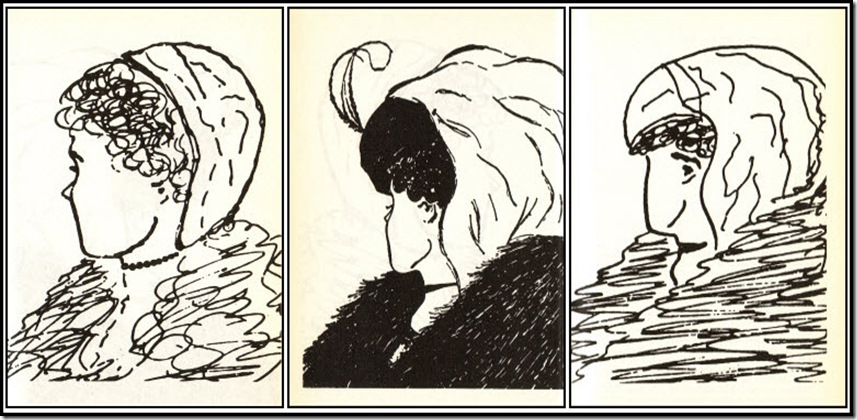
\includegraphics[width=0.95\textwidth]{zdroje/POV-both.jpg}
\caption{Třetí obrázek pro porovnání}
\end{figure}


\pagelogos
\end{document}
